\documentclass{imcs}
\usepackage[T2A]{fontenc}
\usepackage[utf8x]{inputenc}
\usepackage[russian]{babel}
\usepackage{graphicx}
\usepackage{hyperref}
\usepackage{enumitem}
\usepackage{listings}
\usepackage{courier}

\lstset{basicstyle=\footnotesize\ttfamily,breaklines=true}



\makeatletter
\let\old@itemize=\itemize
\def\itemize{\old@itemize
\setlength{\itemsep}{10pt}
\setlength{\parskip}{0pt}
\setlength{\leftskip}{0pt}
}
\makeatother

\makeatletter
\let\old@enumerate=\enumerate
\def\enumerate{\old@enumerate
\setlength{\itemsep}{10pt}
\setlength{\parskip}{0pt}
\setlength{\leftskip}{0pt}
}\makeatother

\title{Модуль контролируемого исполнения программ Spawner}
\author{Храпченков Пётр Фёдорович}
\mentorinfo{старший преподаватель}
\mentorname{А.С.~Кленин}
\year{2014}



\begin{document}
\maketitle

\tableofcontents
\pagebreak

\section*{Аннотация}
\addcontentsline{toc}{section}{Аннотация}
Цель данной работы - реализовать поддержку замыканий в компиляторе Free Pascal Compiler.
Рассмотрены подходы к решению проблемы и осуществлена реализация.
Модуль Spawner является частью автоматической проверяющей системы CATS и используется для запуска программ с ограничениями на использование системных ресурсов и получения информации об использованных системных ресурсов программой, а так же информации о ходе исполнения.

В рамках данной работы проводилась интеграция в систему CATS.

\pagebreak

\section{Введение}
\subsection{Глоссарий}

Системные ресурсы -- Набор системных ресурсов включает в себя время исполнения программы в пользовательском режиме, физическое время исполнения, объем выделенной памяти, объем записанной на диск информации.

Физическое время исполнения -- абсолютное время, определяемое глобальным системным таймером.

Уровень загрузки -- величина, отображающая отношение времени в пользовательском режиме к физическому времени.

Время простоя -- время, в течении которого уровень загрузки программы находился не выше установленного минимального.

Sandboxing -- в компьютерной безопасности защитный механизм для изолированного исполнения программ. Часто используется для запуска непроверенного кода или сомнительных программ от неизвестных разработчиков, поставщиков, подозрительных пользователей или веб сайтов.

JOB\_OBJECT -- это объект, способный иметь имя, настройки безопасности, который контролирует атрибуты ассоциированных с ними процессов. Операции, применяемые к ним, влияют на все процессы, включенные в него. Так, например можно ограничить память, приоритет процессов, а так же завершить их все.

Анонимная функция (англ. anonymous function) -- функция, не имеющая идентификатора; доступна для
вызова либо в момент создания, либо, позднее, через ссылку на функцию,
хранящуюся в переменной.

Анонимный метод (англ. anonymous method) -- реализация замыканий в языке программирования Delphi\cite{anonymmethods}. 

Замыкание (англ. closure) -- функция или ссылка на функцию вместе с используемым ею
окружением; замыкание сохраняет окружение и позволяет функции
обращаться к нему даже если она вызвана за пределами лексического
контекста, где была создана.

Захваченная переменная (англ. captured variable) -- переменная, используемая в теле замыкания,
объявленная во внешнем для замыкания лексическом контексте.

Интерфейс с подсчётом ссылок (англ. reference counted interface) -- набор функций, используемый компилятором для
автоматического управления памятью объектов. Класс, реализующий такой интерфейс,
становятся управляемым типом данных.

Область видимости объявления (англ. scope) -- область программы, в которой может 
использоваться это объявление.

Сборщик мусора (англ. garbage collector) -- часть библиотеки времени исполнения, отвечающая за освобождение
динамической памяти, занятой недостижимыми данными.

Свободная переменная (англ. free variable) -- переменная, используемая в теле функции, но не
являющейся параметром или локальной переменной этой функции.

Управляемый тип данных (англ. managed type) -- тип данных, для которого компилятор
использует специальные техники управления динамической памятью,
такие как подсчёт ссылок\cite{delhpimanged}.

Функциональное программирование -- парадигма программирования,
рассматривающая вычисление как применение математических функций,
отрицающая понятие состояния и изменяемых данных.


\subsection{Описание предметной области}

На сегодняшний день в России и мире проводится множество соревнований по программированию, включая известный командный чемпионат мира по программированию среди студентов высших учебных заведений АСМ (1), а так же олимпиады школьников по информатике. Обычно при подготовке подобных соревнований разрабатываются пакеты заданий, состоящие из формулировки задачи, условий к входным и выходным данным,  набора тестов, а так же эталонного решения. Для проведения соревнования используются различного рода автоматизированные системы, использующий полученные пакеты заданий. Такие системы предоставляют удобный интерфейс: для участников – просмотра и отправки своих решений, для организаторов – создание соревнований, а так же наблюдения за их ходом.
В частности, одной из таких систем является автоматическая система проведения соревнований CATS (2). Система разрабатывалась на базе ДВФУ и успешно применялась при проведении различных турниров. Она состоит из веб-интерфейса, базы данных, а так же модуля judge.
Веб интерфейс предоставляет возможность участвовать в доступных турнирах, просматривать задачи, отправлять соответствующие решения, выполненные в разрешенных системой (турниром) средах разработки, следить за ходом их тестирования, следить за ходом турнира и др. Для организаторов, в свою очередь, веб-интерфейс позволяет создавать турниры, добавлять в них задачи, следить за ходом турнира и др.
Связь между веб интерфейсом и модулем judge осуществляется через базу данных. [2] Веб интерфейс и база данных являются кросс-платформенными составляющими системы и могут быть установлены на компьютеры под управлением различных операционных систем.
Модуль judge использует Spawner для исполнения программ участников с контролем безопасности и ограничений на системные ресурсы. Он представляет собой набор скриптовых утилит, который занимается сборкой и тестированием решений участников и последующей отправкой результата в базу данных (подробнее см. раздел Архитектура).
Модуль Spawner разрабатывался как часть системы CATS и имел достаточный для этого функционал. Однако, с появлением новых типов задач, таких как интерактивные (3) в соревнования вроде Всероссийской олимпиады школьников по информатике стала очевидной необходимость расширения модуля. Так же, на базе ДВФУ неоднократно проводились соревнования искусственного интеллекта, где тоже требуется контролируемое исполнение программ участников, что вместе с предыдущим пунктом поставило задачу множественного исполнения. Дополнительно, консольная утилита Spawner оказалась несовместимой с 64 разрядными операционными системами Windows, в силу специфики кода. К тому же, модуль Spawner являясь чистым Windows приложением не позволяет проводить более тесную интеграцию веб-сервера с модулем judge. Можно дополнить, что другие подобные модули реализуют более расширенный функционал, например, по вводу новых ограничений, таких как ограничение на время простоя. А вследствие отсутствия финальной версии исходного кода нет возможности проводить дальнейшие изменения и улучшения.
Таким образом, перечисленные выше пункты послужили мотивацией к написанию данной работы.

\subsection{Неформальная постановка задачи}

Требуется доработать модуль Spawner для выполнения следующих требований:
•	Полная совместимость с предыдущей версией Spawner’а для внедрения в систему CATS.
•	Проверка на наличие и корректная обработка исключений, возникших во время работы программы.
o	Борьба с гуи исключениями
•	Ограничения на использование подконтрольной программой системных ресурсов:
o	память
o	время работы
o	время исполнения
o	запись в файлы
o	время простоя
•	Вывод отчета в других форматах, включая как json, так и форматы отчетов других подобных модулей
•	Кроссплатформенность
o	Возможность работы системы как в 32 так и в 64 битном окружении системы Windows.
o	Дальнейшая разработка совместимых версий для Linux и др.
•	Работа со стандартными потоками - stdin, stdout и stderr, их перенаправление
•	Корректный запуск программ из-под заданного пользователя.
•	Множественное исполнение программ
o	Перенаправление потоков ввода/вывода
o	Поддержка ролей запускаемых процессов
•	Анализ и дополнение существующего формата входных аргументов, соответствующего указанным выше требованиям
•	Интеграция доработок в систему CATS
•	Возможность отдельного использования функционала утилиты в виде библиотеки.

\iffalse OLD:
Добавить в компилятор Free Pascal поддержку замыканий. В режиме совместимости с 
Delphi реализация должна вести себя так же, как и анонимные методы
Delphi. Дополнительно рассмотреть возможность создания альтернативной улучшенной
реализации, не ограниченной требованием совместимости с Delphi.
При этом компилятор должен сохранить обратную совместимость, проходить существующие тесты. 

\subsubsection{Анонимные подпрограммы}

В некоторых языках программирования, анонимные функции - единственный
способ создать замыкание. Тем не менее эти понятия не тождественны.
Анонимная функция - это функция не имеющая идентефикатора. Существуют
языки программирования, поддерживающие анонимные функции, но не
поддерживающие замыкания. Компилятор FPC должен поддерживать
объявление анонимных функций в теле других подпрограмм:
\begin{lstlisting}
function Factory: TProc;
begin
  Result := procedure begin
              Writeln('executed');
            end;
end;
\end{lstlisting}

\subsubsection{Вложенные функции}

Вложенная функция может обращаться к переменным объемлющих функций. Некоторые
языки программирования позволяют создавать замыкания при помощи вложенных анонимных
функций. На данный момент FPC и Delphi поддерживают вложенные именованные функции, но
не позволяют создавать с ними замыкания. Без поддержки замыканий ссылка на вложенную
функцию не сохраняет окружение. Это значит, что вложенную подпрограмму нельзя вызывать 
по сохранённой ссылке после того, как работа объемлющей подпрограммы завершилась.
Для обратной совместимости семантика вложенных подпрограмм должна остаться неизменной.
Вложенные процедуры не должны создавать замыкания. В дальнейшем возможно создание
нового синтаксиса для создания замыканий с использованием вложенных именованных функций.

Ниже приведён пример вложенной функции, использующей переменную объемлющей функции.
Использование ссылки на вложенную функцию после окончания работы объемлющей подпрограммы,
в которой была создана эта ссылка, является ошибкой.
\begin{lstlisting}    
procedure outer;
var i: Integer;

  procedure inner; begin
    i := 10;
  end;

begin
  ...
end;    
\end{lstlisting}

\subsubsection{Продление жизни локальных переменных}

Замыкание в момент создания сохраняет используемое окружение.
Типичной является ситуация, когда замыкание использует локальные переменные
объемлющей функции. Без поддержки замыканий время жизни локальных
переменных ограничено временем выполнения функции, где она объявлена.
Время жизни переменной, захваченной из замыкания заканчивается только
когда не осталось использующих её замыканий.

Ниже приведён пример анонимной функции, использующей переменную объемлющей функции.
Без замыканий переменная data стала бы недоступной после завершения
работы функции Factory. Замыкание продлевают жизнь захваченной переменной data, и может
обращаться к ней даже после окончания работы функции Factory. В момент второго
вызова процедуры Factory переменная data, захваченная первым замыканием, покинула зону видимости. 
Теперь она доступна только ссылающемуся на неё замыканию. Следующий вызов Factory создаст
другое замыкание, ссылающееся на другую переменную data.
Каждое из созданных замыканий хранит ссылку на свой собственный
экземпляр захваченной переменной. Вызов f1() напечатает значение 10, а вызов f2()
напечатает 20.
\begin{lstlisting}
function Factory(data: Integer): TProc;
begin
  Result := procedure
            begin
              Writeln( data );
            end;
  end;
    
var f1: TProc;
begin
  f1 := Factory(10);
  f2 := Factory(20);
  f1();               { 10 }
  f2();               { 20 }
end.
\end{lstlisting}    

\subsubsection{Захват по ссылке}

В языке программирования Delphi замыкания захватывают переменные по ссылке. Необходимо
реализовать такой же подход. Для захвата по ссылке типична ситуация, 
когда захваченную замыканием переменную меняют из другого замыкания,
или из обычной подпрограммы. Приведённый ниже код демонстрирует, как сразу два созданных
замыкания используют одну и ту же переменную. Кроме того, захваченная переменная
используется в теле функции, где она объявлена.
\begin{lstlisting}
type TProcInt: reference to procedure(n: Integer);
     TProc: reference to procedure; 
var data: Integer;
    pset: TProcInt;
    pget: TProc;
begin
  pset := procedure(n: Integer) begin 
            data := n;
          end;
  pget := procedure begin
            Writeln(data);
          end;
  data := 0;
  pget();                {  0 }
  pset(10);
  pget();                { 10 }
end.
\end{lstlisting}

\subsubsection{Захват по значению}
Рассмотреть возможность реализации захвата по значению. Пример ниже демонстрирует 
возможный синтаксис, позволяющий явно указывать, как захватывать переменные: по
ссылке или по значению. За описанием сигнатуры функции следует описание
захваченных переменных. После ключевого плова closure в круглых скобках через запятую
указываются имена захваченных по значению переменных. Остальные переменных, используемые в
теле функции захватываются по ссылке. 
\begin{lstlisting}
var i: Integer;
    f: TProc;
begin
  i := 0;
  f := procedure
       closure(i)
       begin
         Writeln(i);
       end;
  i := 10;
  f();                { 0 }
end.
\end{lstlisting}

\iffalse TODO: в качестве исключения описать здесь дискуссию из мейлинг листа
по этому поводу \fi

\subsubsection{Упрощенный синтаксис}
Рассмотреть возможность реализации упрощенного синтаксиса для более лаконичного объявления
анонимных функций. В примере ниже в метод map передаётся анонимная функция, принимающая
один аргумент типа Integer и возвращающая значение аргумента, увеличенное на 1.
\begin{lstlisting}
type TListVisitor = function(x: Integer): Integer;
var  list: TIntList;
begin
   ...
   list.map(TListVisitor is x + 1)
   ...
end.
\end{lstlisting}
\fi

\subsection{Обзор существующих методов решения}

\subsubsection{Аналогичные решения}

\iffalse TODO: добавить JAVA, Scala \fi
\iffalse TODO: посмотреть с какой версии поддерживается та или иная фича, показать что замыкания совсем недавно появились во многих языках \fi

Следующие системы тестирования включают в себя модули подобные реализуемому в данном проекте spawner’у
ejudge http://ejudge.ru/   
ejudge - это система для проведения различных мероприятий, в которых необходима автоматическая проверка программ. Система может применяться для проведения олимпиад,
поддержки учебных курсов и т.д.
Для контроля исполнения используется патч к ядру Linux. Модуль контроля исполнения программ представляет собой набор скриптов. Невозможно портирование скриптов на ОС Windows в силу их зависимости от системных функций.
PCMS2/Run http://neerc.ifmo.ru/trains/information/software.html
PCMS2(Programming Contest Management System)
Система контроля исполнения представляет собой консольную утилиту. Используется динамическая библиотека. Для создания и контроля исполнения процесса от другого пользователя требуются особые привилегии.
Во многом схожий проект, однако для запуска программ постоянно используется режим отладки.
Contester
Contester - это система для проведения турниров и индивидуального решения задач по олимпиадному программированию (спортивному программированию). Система содержит условия задач - от легких до олимпиадных - и возможность проверки решений на большинстве современных языков: C++, Object Pascal, Java и языках .NET: C\#, J\# и Visual Basic.
Не тестировалось.
Executor http://acmtest.ru/
Executor - автоматизированная сетевая тестирующая система для проведения турниров по программированию по правилам ACM. Executor - freeware, распространяется бесплатно и без каких-либо ограничений на использование.
Тестирование контроля исполнения не производилось
PC² http://www.ecs.csus.edu/pc2/
PC²(Programming Contest Control System) - система разработанная в Калифорнийском Государственном Университете Sacramento (CSUS) в поддержку соревнований по программированию, проводимых ACM и, в частности, ACM International Collegiate Programming Contest (ICPC) и его региональных этапов. 
Контроль исполнения, как неотъемлемая часть общей системы.
olympiads.ru/RUN http://olympiads.ru/school/system/index.shtml
Система самотестирования olympiads.ru. Используется для тестирования решений задач, представленных на соответствующем сайте. Система работает на платформе Windows, имеет инсталляционную программу и документацию. 
Вследствие того что система не поддерживается с 2003 года и имеет узкий функционал в рамках данной работы детально рассматриваться не будет.
DOMjudge http://domjudge.sourceforge.net/
DOMjudge - автоматизированная тестирующая система, для проведения соревнований по программированию, подобных ACM ICPC. Основной упор сделан на удобство использования и безопасность. Система участвовала во многих соревнованиях, распространяется свободно на условиях открытого ПО. 
Для контроля исполнения используется набор небольших консольных утилит.
dudge http://code.google.com/p/dudge/
Dudge - это универсальная система для проведения олимпиад по программированию и другим предметам, написанная на Java и J2EE с использованием СУБД PostgresSQL и распространяющаяся по лицензии GPL. 
В качестве контроля исполнения используется динамическая библиотека, реализована для Windows и Unix. Библиотека используется в Java коде. Для создания и контроля исполнения процесса от другого пользователя требуются особые привилегии.(не подтверждено)
cats-judge/Spawner прототип http://imcs.dvgu.ru/cats/docs/spawner.html
cats-judge - автоматизированная тестирующая система, для проведения как одиночных, так и командных соревнований по программированию.
Для контроля исполнения используется консольная утилита. Создание и контроль исполнения процесса от другого пользователя требуют особые привилегии.
Spawner http://code.google.com/p/spawner/
Дальнейшее развитие модуля контроля запуска и исполнения программ cats-judge/Spawner .
На данный момент представляет собой обратно совместимую консольную утилиту с расширенными, по сравнению с предыдущей версией, возможностями.
Функционал реализован только для систем семейства Windows.

\iffalse OLD:
Ниже приведена таблица, показывающая, какие из популярных языков программирования поддерживают
замыкания. Для языков с замыканиями указано, как именно можно создавать
замыкания. При помощи анонимных функций или вложенных именованных функций.
Так же приведена информация о том, какой способ захвата использует соответствующий язык.
\fi

\begin{table}[h!]
\begin{center}
\begin{tabular}{|l|c|c|c|c|c|c|}
\hline
  Название   &  Операционная  &  Лицензия  &  Интерфейс  &  Язык	 		&  Защищенный запуск 	  & Комментарий \\
         	&  система    	 &      		  &  	   		&  реализации   	& под другим пользователем &	           \\
\hline
 Perl    &  +          &  +/-        &             &  +          &  +   &   -    \\
\hline
\end{tabular}
\caption{Поддержка замыканий и анонимных функций современными ЯП}\label{tab:wsi_diff_rel}
\end{center}
\end{table}
 
\iffalse OLD: 
 
\begin{table}[h!]
\begin{center}
\begin{tabular}{|l|c|c|c|c|c|}
\hline
  ЯП     &  Анонимные  &  Вложенные  &  Захват по  &  Захват по  &  Замыкания  \\
         &  функции    &  функции    &  значению   &  ссылке     &             \\
\hline
 Perl    &  +          &  +/-        &             &  +          &  +          \\
\hline
 Python  &  +          &  +          &             &  +          &  +          \\
\hline
 Ruby    &  +          &  +          &             &  +          &  +          \\
\hline
 Scheme  &  +          &  +          &             &  +          &  +          \\
\hline
 Elisp   &  +          &  +          &             &  +/-        &             \\
\hline
 Scala   &  +          &  +          &             &  +          &  +          \\
\hline
 Java    &             &             &             &  +          &  +/-        \\
\hline
 C       &             &             &             &             &             \\
\hline
 C++     &  +          &             &  +          &  +/-        &  +          \\
\hline
 Delphi  &  +          &  +          &             &  +          &  +          \\
\hline
 Fpc     &             &  +          &             &             &             \\
\hline
\end{tabular}
\caption{Поддержка замыканий и анонимных функций современными ЯП}\label{tab:wsi_diff_rel}
\end{center}
\end{table}


Некоторые языки имеют особенности, помеченные в таблице знаком +/-.
Язык программирования Перл позволяет объявлять вложенные функции, но к ним не применяются обычные правила
статической области видимости переменных. Язык программирования Elisp имеет динамическую область 
видимости переменных. Java позволяет объявлять анонимные классы, содержащие именованные методы, но не 
позволяет объявлять анонимные функции. С++ предоставляет синтаксис для доступа к переменным по ссылке,
но не продлевает жизнь захваченным переменным.

Сегодня большинство популярных языков программирования поддерживают
замыкания. В некоторые языки они были добавлены недавно. К
примеру, в стандарт с++ замыкания попали в 2011м году. В Java
полная поддержка замыканий станет доступной в версии Java 8,
запланированной на середину текущего года.
\fi

\subsubsection{Описание предшествующих работ}
Студенты нашей кафедры успешно развивали компилятор Fpc в рамках своих
курсовых и дипломных работ:
\begin{enumerate}
    \item Дипломная работа «Расширение компилятора Free Pascal для поддержки обобщённого программирования». Автор Нелепа А.А. Руководитель Кленин А. С. 2007г.\cite{diplomnelepa}
    \item Курсовая работа «Анализ потоков управления для языка программирования Pascal» Автор Баль Н.В. Руководитель Кленин А.С. 2008г.\cite{coursebal}
    \item Курсовая работа «Доработка компилятора Free Pascal: case of string» Автор Денисенко М.В. Руководитель Кленин А.С. 2009г.\cite{misha}
    \item Курсовая работа «Оператор for-in для компилятора Free Pascal» Автор Лукащук М.А. Руководитель Кленин А.С. 2010г.\cite{courseluck}
\end{enumerate}

\subsubsection{Вывод}

Ценность замыканий подтверждена их популярностью и востребованностью. 
Сегодня замыкания поддерживают большинство языков программирования, а программисты 
активно используют их на практике. Поэтому для поддержания компилятора FPC в 
актуальном состоянии необходимо реализовать в нём поддержку замыканий.

\subsection{План работ}

\begin{enumerate}
    \item Согласовать работу с разработчиками FPC.
    \item Изучить архитектуру и исходных код компилятора.
    \item Изучить реализацию замыканий в похожих языках программирования.
    \item Спроектировать реализацию.
    \item Поэтапно осуществить реализацию:
      \begin{itemize}
          \item Добавить возможность объявлять анонимные функции. Запретить захват переменных.
          \item Добавить возможность захвата переменных функции, объявляющей замыкание.
          \item Добавить возможность захвата любых локальных переменных, 
                доступных в текущем лексическом контексте\footnote{За исключением случаев, описанных в разделе "Функциональные требования".}.
      \end{itemize}        
\end{enumerate}

\section{Требования к окружению}

\subsection{Требования к аппаратному обеспечению}

Для работы требуется компьютер, пригодный для компиляции исходного кода программы или исполнения существующих пакетов.
Т.е. кроме работающих процессора, оперативной и постоянной памяти требуются
клавиатура и монитор.

Поддерживаемые архитектуры процессоров\cite{fpctargets}:
\begin{itemize}
    \item I386
    \item PowerPC
    \item Sparc
    \item AMD64 (x86-64)
    \item PowerPC64
    \item ARM
    \item m68k 
\end{itemize}

\subsection{Требования к программному обеспечению}

\subsubsection{Операционная система}
\begin{itemize}
    \item Windows не ниже ХР
    \item Linux
\end{itemize}

\subsubsection{Компилятор} 
\begin{itemize}
    \item Microsoft Visual Studio 2005 и новее или G++ 4.7.7 и новее
    \item CMake 2.6 и новее
\end{itemize}
    
\subsection{Требования к пользователям}
Программисты, владеющие языком программирования Free Pascal или Delphi.

\section{Архитектура системы}

Несмотря на то, что для конечного пользователя автоматизированная система представлена в виде Web интерфейса, она является аппаратно-програмным комплексом, состоящим из нескольких модулей.
В рамках данной работы необходимо рассмотреть внутреннее устройство системы, для обоснования некоторых принятых решений.
\iffalse TODO: каких? \fi

\subsection{Архитектура системы CATS}
Автоматизированная система CATS состоит из нескольких частей: веб интерфейс, база данных, а так же модуль judge. В базе данных системы хранятся данные о проводимых турнирах, пакеты задач, информацию б участниках, их попытках, а так же информация по средам разработки.

Весь программный код можно условно разделить на начальную стадию(англ. front-end)
и заключительная стадию(англ. back-end)\cite{dragonbook}.

Начальная стадия считывает входные данные, проверяет их на корректность, строит
вспомогательные структуры данных, необходимые для генерации кода и передаёт 
управление заключительной стадии, которая генерирует код.

Смысл разделения на начальную и заключительную стадию в
том, чтобы отделить детали анализа языков высокого уровня от деталей,
относящихся к целевой архитектуре. Такой подход позволяет уменьшить сложности
одновременной поддержки несколько диалектов Pascal и большого числа целевых
архитектур.

\subsubsection{Начальная стадия}

После запуска FPC обрабатывает параметры и проводит предварительную обработку
исходного кода входной программы. Далее он целиком считывает определение и тело
одной подпрограммы, проводит необходимые проверки и генерирует для неё
код высокоуровневого ассемблера. Затем считывает следующую подпрограмму и так далее
до конца файла.

Обработка одной подпрограммы на начальной стадии включает в себя:
\begin{enumerate}
    \item Лексический анализ.
    \item Синтаксический анализ.
    \item Семантический анализ.
    \item Машинно-независимую оптимизацию.
\end{enumerate}

Операции, производимые любым компилятором можно реализовывать в виде
отдельных проходов по синтаксическому дереву или потоку лексем. К примеру, можно
полностью считать лексемы входного файла и получить поток лексем. Затем запустить
синтаксический анализ и получить синтаксическое дерево, соответствующее содержимому
файла. Затем семантический анализ, который не производит никаких модификаций и 
лишь проверяет синтаксическое дерево на корректность. И лишь потом производить
преобразования синтаксического дерева.

Описанная выше схема уменьшает сложность исходного кода компилятора. Программу, в которой отдельные 
компоненты совершают чётко определённые действия легко документировать и понимать.
К сожалению, многократный обход структур данных, расположенных в памяти непоследовательно,
вносит накладные расходы\cite{kaspersky}, поэтому
зачастую несколько отдельных проходов объединяют в один. В компиляторе FPC стадии
лексического, синтаксического и семантического анализа реализованы в виде одного
прохода. 

Кроме того, стадия семантического анализа, кроме вывода типов и проверки синтаксического
дерева на корректность, производит вспомогательные модификации синтаксического дерева.
FPC на этапе семантического анализа добавляет преобразования типов, заменяет операции
с управляемыми данными на вызовы функций из библиотеки времени исполнения и трансформирует
некоторые специфичные конструкции. К примеру, для загрузки адреса процедуры вставляется
специальный узел синтаксического дерева, отличный от созданного лексическим анализатором.

\subsubsection{Синтаксическое дерево}

Синтаксическое дерево - иерархическая структура данных представляющая синтаксическую
структуру исходной программы\cite{dragonbook}. После синтаксического анализа каждый внутренний узел 
дерева представляет собой оператор, дочерние узлы представляют собой операнды этого
оператора. Для представления синтаксического дерева и операций над ним FPC использует
приём объектно-ориентированной декомпозиции. В \cite{gof} такой подход описан под
названием "composite"(англ. составной).

Все узлы синтаксического дерева унаследованы от одного абстрактного класс tnode.
tnode объявляет общий интерфейс для объектов синтаксического дерева. Унаследованные
от tnode классы, реализуя этот интерфейс, определяют специфичное поведение. Отметим
методы, реализующие обходы синтаксического дерева:
\begin{itemize}
    \item pass\_1 -- выделение регистров;
    \item pass\_typecheck -- семантический анализ;
    \item pass\_generate\_code -- генерация кода.
\end{itemize}

На рис.~\ref{tcgloadvmtaddrnode} приведён пример того, как использование
наследования позволяет отделить общие для 
нескольких синтаксических конструкций детали от специфичных деталей отдельной конструкции.
Так, tunarynode служит базовым классом для всех операций, содержащих 1 операнд.
Унаследованный от него класс tloadvmtaddrnode реализует методы pass\_1 и pass\_typecheck,
которые реализованы без использования информации о целевой архитектуре. Метод
генерации кода pass\_generate\_code реализован в классе \\ tcgloadvmtaddrnode.

Таким образом, для каждой архитектуры процессора можно создать отдельный класс, 
унаследованный от tloadvmtaddrnode и реализовать генерацию кода, 
учитывая особенности конкретного процессора.
Такой подход к модификации поведения объекта, переопределяя методы родительского класса,
описан в \cite{gof} под названием "template"(англ. шаблон). Этот подход широко
используется в FPC для отделений специфичных деталей генерации кода для узлов синтаксического
дерева от остальной логики.

\begin{figure}[htb]
\centering
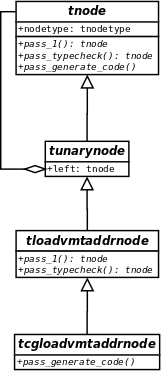
\includegraphics{./uml/cgnodeexample.png}
\caption{Диаграмма наследования для класса tcgloadvmtaddrnode}
\label{tcgloadvmtaddrnode}
\end{figure}

\pagebreak

\subsubsection{Таблицы символов}

Таблица символов это структура данных, которая используется компилятором для хранения 
информации о именованных объектах программы. Такая информация последовательно накапливается во время
разбора синтаксических конструкций. Далее она используется на этапе семантического анализа 
для проверки соответствия типов и при генерации кода для размещения данных в памяти.

Записи в таблице символов содержат символьные строки, типы, области видимости, 
местоположение в памяти и прочую связанную с именованными объектами информацию.
FPC использует таблицы символов для хранения информации о модулях,
константах и переменных, подпрограммах, структуре составных типов данных.

Таблицы символов и синтаксическое дерево тесно связаны: синтаксическое дерево описывает действия с
данными. Записи таблицы символов описывают структуру этих данных.

\subsubsection{Трансформации синтаксического дерева}

Во время компиляции FPC неоднократно трансформирует полученное на этапе синтаксического 
анализа синтаксическое дерево. Это необходимо для:
\begin{itemize}
    \item Упрощения логики отдельных узлов синтаксического дерева. К 
примеру, узлы преобразования типов упрощают логику узлов загрузки значения переменных,
арифметических операций и др. выражений.
    \item Проведения машинно - независимой оптимизации. К примеру удаление недостижимого
кода.
    \item Реализации новых концепций языка через старые. Примерами являются реализация
case of string\cite{misha} а так же доступ к локальным переменным объемлющей функции для
платформ, не поддерживающих арифметику указателей.
\end{itemize}      

Возможность реализации новых концепций языка через старые можно использовать и
для реализации замыканий. Заметим, что замыкание отличается от 
обычной подпрограммы наличием сохранённого состояния свободных переменных. Преобразование
замыкания в функцию, не содержащую свободных переменных, называется преобразованием
замыканий\cite{moderncompiler}.

Преобразование замыканий давно используется в языках программирования, основанных на
лямбда-исчислении. Прямая реализация модели подстановки
лямбда-исчисления приводит к многократному вычислению одних и тех же выражений.
Преобразованием замыканий позволяет таким языкам избежать бесполезных вычислений
и улучшения производительности программ \cite{lambdaclosure95}. 
Функция со свободными переменными
заменяется функцией с дополнительными параметром - окружением. Свободные переменные
в теле исходной функции заменятся ссылками на окружение.  
Неизменяемость переменных в лямбда - исчислении позволяет реализовать сохранение
переменных в окружение разными способами:

\iffalse TODO: руководителю не понравились эти пироги. Рассказать про наш случай, плевать
на функциональные языки.

\begin{description}
    \item[Общее окружение] Замыкания, имеющие общие свободные переменные,
используют общее окружение. Во время выполнения программы по мере активации функций
из вновь созданных окружений необходимо составлять связный список.
Преимущество такого подхода -- быстрое создание окружения и экономия памяти. Недостатком
является увеличение времени доступа к переменным, т.к. время доступа к элементам
окружения пропорционально уровню вложенности функции.
    \item[Плоское окружение] Для каждого замыкания создаётся отдельная структура данных,
содержащая значения всех необходимых переменных. Плюс такого подхода -- быстрый доступ
к переменным окружения. Минус - долгое создание замыкания и дополнительный расход памяти.
\end{description}

\fi

Преобразование замыканий применимо и к императивным языкам
программирования. Статически типизированный язык программирования Scala
использует преобразования замыканий\cite{scalaoverview}\cite{scalaclosure}.
Scala имеет статическую типизацию и допускает изменение значения переменных. Этом
язык очень похожим на Free Pascal. Главное отличие -- полностью автоматическое
управление динамической памяти компилятором, решающее проблему управления памятью
созданных окружений.

\subsubsection{Заключительная стадия}

В FPC нет промежуточного представления кода, который начальная стадия
передавала бы в заключительную стадию. Вместо генерации промежуточного представления
начальная стадия во время обхода синтаксического дерева последовательно вызывают методы
высокоуровневого генератора кода. Такой подход очень похож на использование
промежуточного представления, но избавляет от необходимости генерировать промежуточные
структуры данных.

\iffalse TODO: рассказать почему генератор высокоуровневый и зачем здесь диаграмма. \fi

\begin{figure}[htb]
\centering
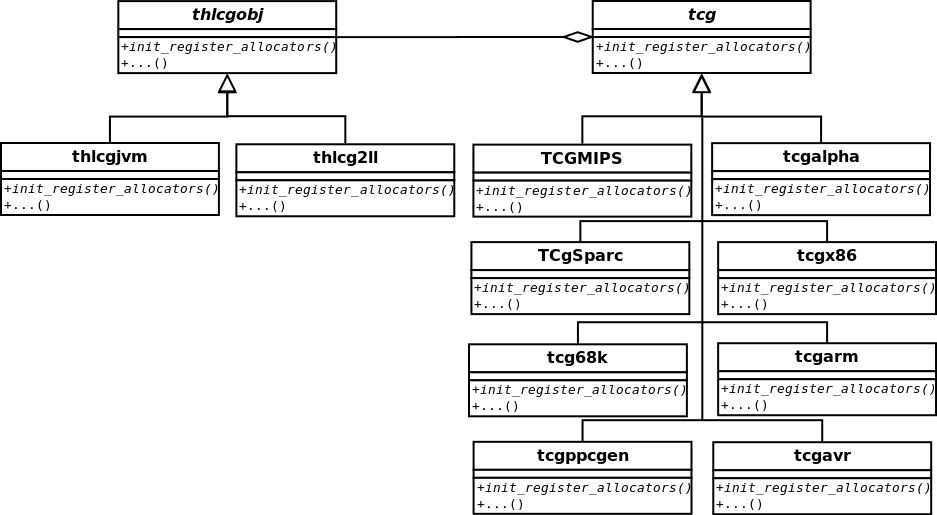
\includegraphics{./uml/cgen.png}
\caption{Диаграмма классов генератора кода}
\end{figure}

\pagebreak

\section{Функциональные требования}

Компилятор должен:
\begin{enumerate}
    \item Позволять объявлять анонимные подпрограммы внутри тела других подпрограмм. В том числе с любым уровнем
вложенности. Синтаксис объявления анонимной подпрограммы такой же как и для обычной подпрограммы, с двумя
исключениями:
        \begin{itemize}
            \item после ключевых слов procedure и function нет идентификатора, а сразу идет опциональный список формальных аргументов;
            \item после списка формальных аргументов (если он опущен, то после ключевых слов procedure или function) не ставится точка с запятой.
        \end{itemize}

         Пример 1:
\begin{lstlisting}
  procedure begin
    Writeln('inside');
  end;
\end{lstlisting}

         Пример 2:
\begin{lstlisting}
  procedure begin
    Writeln('inside');
  end;
\end{lstlisting}

    \item Позволять анонимным функциям возвращать значения, используя ключевое слово Result:

Пример:
\begin{lstlisting}
  function(num: Integer): Integer begin
    Result := num + 10;
  end;
\end{lstlisting}

    \item Запрещать анонимным процедурам использовать переменную Result объемлющей функции:

Пример:
\begin{lstlisting}
  function Calculate: Integer;
  begin
    ...
    procedure begin
      Result := 10; // Error, result can't be captured
    end;
  end;
\end{lstlisting}

    \item Запрещать анонимным процедурам использовать параметры объемлющей функции, объявленные с модификатором
var или out.

\iffalse TODO: улучшить \fi

    \item Запрещать анонимным процедурам использовать переменные, объявленных в обработчике исключений.

\iffalse TODO: улучшить \fi

    \item Позволять анонимным процедурам использовать переменные, объявленные в объемлющей функции:

Пример:
\begin{lstlisting}
  procedure Calculate: Integer;
  var num: Integer;
  begin
    ...
    procedure begin
      num := 10;
    end;
  end;
\end{lstlisting}

    \item Позволять анонимным процедурам использовать переменные, объявленные в объемлющей функции, при уровне вложенности больше 1:

Пример:
\begin{lstlisting}
  procedure Outer;
  var num: Integer;
    procedure Calculate;
    begin
      ...
      procedure begin
        num := 10;
      end;
    end;
  begin
   ...
\end{lstlisting}

    \item Продлевать время жизни захваченных переменных. Время жизни захваченной переменной определяется не временем работы функции, где она объявлена, а временем жизни всех ссылающихся на неё замыканий.

    \item Управлять памятью замыканий автоматически, используя счётчик ссылок. Время жизни замыкания заканчивается
 только, когда не остаётся указателей соответствующего типа, ссылающихся на это замыкание.
      
    \item Осуществлять захват переменных по ссылке. Замыкания, созданные в одном лексическом контексте должны иметь доступ к одним и тем же переменным.
      
    \item Корректно осуществлять проверку типов в момент присваивания значений переменным-указателям на замыкание. Это значит, что:
        \begin{itemize}
            \item Переменной можно присваивать определение анонимной функции, если сигнатура анонимной функции
совпадает с сигнатурой, указанной в определении типа переменной. Другими словами, в этом случае используется
структурная эквивалентность выражений, т.к. определение анонимной функции не содержит имя типа.
            \item Переменной можно присваивать значение другой переменной, только если имена типов этих переменных
совпадают. Т.е. в этом случае используется именная эквивалентность выражений.
        \end{itemize}

\iffalse TODO: примерчики \fi
        
      \item Корректно осуществлять проверку типов, если замыкание определено в качестве фактического параметра.
В этом случае так же используется структурная эквивалентность выражений, т.к. определение анонимной функции не
содержит имя типа.

\iffalse TODO: примерчики \fi
        
    \item Предоставлять для вызова замыкания синтаксис аналогичный синтаксису вызова обычных указателей
 на функцию:
        \begin{itemize}
          \item Если замыкание имеет непустой список аргументов, то для вызова в имени переменной-указателя
в круглых скобках добавляется список фактических параметров, разделённых запятыми.
          \item Если замыкание имеет пустой список параметров, то в выражении, состоящем только из вызова
замыкания круглые скобки не содержащие аргументов можно опустить.

\iffalse TODO: примерчики \fi
        \end{itemize}
        
  \item Корректно осуществлять проверку типов во время вызова замыкания. Это значит, что:
        \begin{itemize}
          \item Количество фактических параметров должно равняться количеству формальных параметров.
          \item Типы фактических параметров должны быть эквивалентны типам формальных параметров.
        \end{itemize}

    
\end{enumerate}


\section{Требования к интерфейсу}

Компилятор имеет интерфейс командной строки, который описан
в руководстве пользователя FPC\cite{userguide}. Интерфейс командной строки остаётся неизменным.

\iffalse TODO: это вообще где нужно написать?
Изменения, сделанные в рамках данной работы меняют формат файлов описания модулей. \fi

Введены новые сообщения об ошибках:

\begin{enumerate}
  \item Замыкание не может использовать переменную Result объемлющей функции.
  \item Замыкание не может использовать параметр <имя параметра>, объясленный с модификатором var.
  \item Замыкание не может использовать параметр <имя параметра>, объясленный с модификатором out.
  \item Замыкание не может использовать переменную <имя переменной>, объясленную в обработчике исключений.
  \item Замыкание не может использовать переменную <имя переменной>, объясленную в обработчике исключений.    
\end{enumerate}

Т.к. определение замыкания не содержит имя типа, то существующие сообщения об ошибках вместо имени типа
должны выводить его сигнатуру. Перед сигнатурой функции выводятся ключевые слова ``reference to'', позволяющие
пользователю различить указатель на замыкание от указателя на обычную функцию. К примеру, для кода
приведённого ниже, необходимо вывести сообщение
"Ожидается выражение типа TProc, получено выражение типа reference to procedure(Integer;String)".

\begin{lstlisting}
type TProc = reference to procedure;
var p: TProc;
begin
  p := procedure(i: Integer; b: String) begin end;
end;
\end{lstlisting}

\section{Проект}

\iffalse

\subsection{Средства реализации}

Проект использует язык программирования Free Pascal. Редактирование исходных кодов
компилятора возможно с использованием любого текстового редактора. Тем не менее
для работы с проектом большого размера предпочтительно использование редактора с
поддержкой навигации по коду. Возможность быстрого перехода к объявлению и описанию
идентификаторов упрощает поиск нужной информации и ускоряет процесс разработки.
Было рассмотрено несколько кандидатов:
\begin{description}
  \item[Free Pascal's text mode IDE] Преимущества: находится в репозитории с 
компилятором. Недостатки: отсутствует графический интерфейс, отсутствует
быстрый переход к определению переменных.
  \item[Emacs] Преимущества: мощный текстовый редактор, поддерживающий большое
количество расширений. Недостатки: переход к определению переменных не работает
с исходными кодами Free Pascal.
  \item[Lazarus] Преимущества: удобный графический пользовательский интерфейс.
Корректный быстрый переход к определению символов. Настраиваемые горячие клавиши.
В репозитории компилятора есть файл проекта для Lazarus.
  \item[MSEide] Преимущества: быстрый. Недостатки: неудобный 
пользовательский интерфейс.
\end{description} 
В итоге принято решение использовать среду разработки Lazarus, так как она
лучше всего подходит для работы с большим программным проектом на
языке программирования Free Pascal. Lazarus корректно разбирает
исходный код и предоставляет пользователю возможность удобной и
быстрой навигации по коду.

\fi

\subsection{Структуры данных}

\subsubsection{Базовые структуры данных}

Ключевые структуры данных: определения типов, таблицы символов и
синтаксическое дерево. Программа на языке программирования Free Pascal имеют рекурсивную структуру,
поэтому упомянутые структуры данных имеют сложные циклические зависимости. Пример такой 
зависимости: узел синтаксического дерева, представляющий обращение к переменной содержит имя
переменной. По имени переменной доступен её тип. Типом переменной может быть класс, который
содержит метод. Реализация метода  может содержать обращение к переменной.

\begin{figure}[htb]
\centering
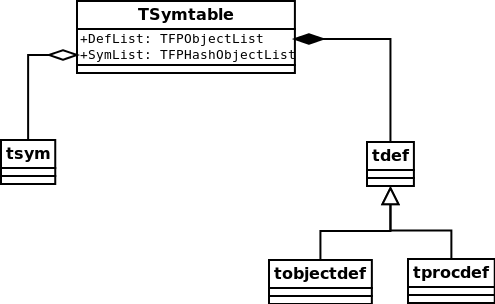
\includegraphics{./uml/sym-def-def-inheritence.png}
\caption{Диаграмма классов}
\label{symboltable-sym-def}
\end{figure}

Таблицы символов отдельно хранят определения типов и символьные имена. Существуют 
различные таблицы символов: таблица символов модуля, локальная таблица символов, таблица
символов с параметрами процедуры и др. Все таблицы символов унаследованы от общего
базового класса TSymTable, определяющего общий интерфейс для работы с ними. Любая таблица символов отдельно
хранит определения типов и литеральные имена, что отражено на рис.~\ref{symboltable-sym-def}.
Таким образом, таблицы символов содержит доступные в текущем лексическом контексте
именованные объекты и соответствующие им типы.

На рис.~\ref{symboltable-sym-def} показаны 2 конкретных класса, унаследованных от
абстрактного класса tdef. Первый из них, tobjectdef, хранит информацию о классе: 
его родитель, реализованные интерфейсы, список методов, список полей и др. Второй, tprocdef, хранит
информацию о типе процедуры: список аргументов, тип возвращаемого значения, локальные
переменные. Отметим, что tprocdef и tobjectdef содержат
список именованных объектов, каждый из которых, тоже имеет тип. Это отражено на
рис.~\ref{symtable-def}, определения типов объекта и процедуры содержат таблицы символов. Причем,
они используют разные конкретные реализации.

\begin{figure}[htb]
\centering
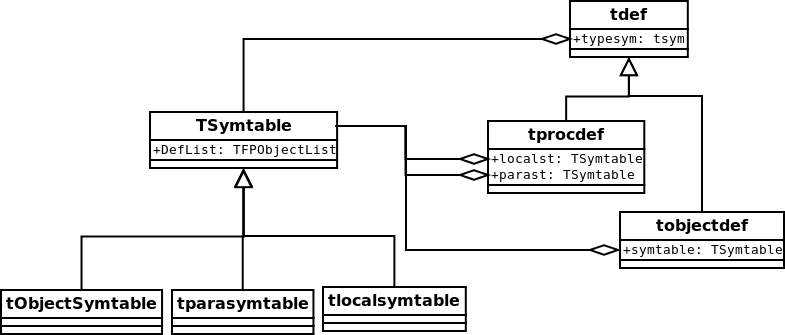
\includegraphics{./uml/symtable-def.png}
\caption{Диаграмма классов}
\label{symtable-def}
\end{figure}

Литеральные имена, используемые для доступа к типам, называются символами. На
рис.~\ref{sym-def-sym-inheritence} изображена диаграмма классов для нескольких символов и 
их связь с определениями типов. Каждый символ унаследован от общего класса tsym. Конкретные
реализации рассчитаны для работы с конкретными определениями типов. 
Из-за того, что Free Pascal поддерживает перегрузку операторов, может существовать несколько
подпрограмм с одним именем и разными определениями. Поэтому tprocsym хранит список ссылок на 
определения типов подпрограмм. В это же время ttypesym содержит только одну ссылку на
определение типа.

\begin{figure}[htb]
\centering
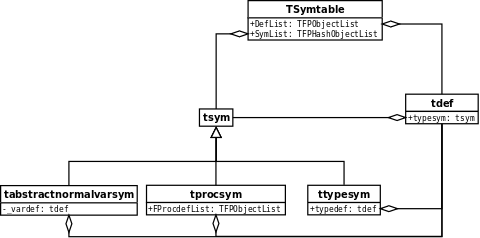
\includegraphics{./uml/sym-def-sym-inheritence.png}
\caption{Диаграмма классов}
\label{sym-def-sym-inheritence}
\end{figure}

Теперь рассмотрим связь синтаксического дерева и таблицы символов. Если таблицы символов отражают
информацию о именованных данных, то синтаксическое дерево отражает информацию о действиях. 
Обращение к переменной является примером действия с именованными данными. Синтаксический
узел, отражающий обращение к переменной - tloadnode. На рис.~\ref{sym-node} показано, как tloadnode
хранит информацию о переменной.

\begin{figure}[htb]
\centering
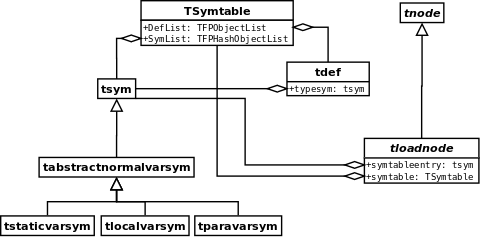
\includegraphics{./uml/sym-node.png}
\caption{Диаграмма классов}
\label{sym-node}
\end{figure}

Кроме ссылок из узлов синтаксического дерева на именованные объекты теоретически возможна обратная
ситуация. Подпрограммы имеют реализацию, которую компилятор обрабатывает в виде синтаксического
дерева. К счастью, определение типа подпрограммы не содержит ссылок на тело подпрограммы. Связь
реализации и информации о типе подпрограммы показана на рис.~\ref{tprocinfo}

\begin{figure}[htb]
\centering
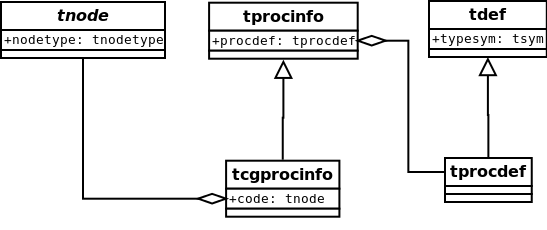
\includegraphics{./uml/tprocinfo.png}
\caption{Диаграмма классов}
\label{tprocinfo}
\end{figure}

\subsubsection{Стек с таблицами символов}

Язык Pascal использует статическую область видимости определений. Это значит, что компилятор
способен узнать область видимости во время компиляции.

Программы и модули на языке Pascal состоят из блоков.
Блок включает в себя объявления меток, констант, типов, переменных и подпрограмм.
Подпрограмма, кроме тела, также может содержать блок. Область видимости объявлений сделанных в блоке
начинается с места их объявления до конца блока\cite{refguide}.
Определения классов и модулей также вносят дополнительные
правила, определяющие области видимости, тем не менее имеющие общие черты с описанными правилами для блоков.

Переменные, объявленные рядом, как правило, имеют общую область видимости. 
Это позволяет эффективно реализовать области видимости
путём настройки отдельной таблицы символов для каждой области видимости\cite{dragonbook}. 
Кроме того, область видимости
объявлений, сделанных во вложенных конструкциях, всегда меньше области видимости объявлений, сделанных
во внешних конструкциях. К примеру, область видимости переменной, объявленной во вложенной функции 
всегда меньше области видимости переменной объемлющей функции. Это позволяет использовать стек для
эффективного управления таблицами символов. 

FPC использует стек с таблицами символов на этапах синтаксического и семантического анализа, а так же во время
проведения трансформаций синтаксического дерева. Таблицы символов, находящиеся на стеке содержат
определения, доступные для использования в текущий момент. Стоит отметить, что без поддержки замыканий
время жизни локальных переменных и их область видимости -- неразделимые понятия. Именно этот факт позволяет
организовать хранилища локальных переменных при помощи стека. Замыкания изменяют время жизни захваченных
локальных переменных, поэтому стек для их хранения не подходит. Так как замыкания не меняют область видимости
локальных переменных, стек таблиц символов по-прежнему остаётся основным инструментом для реализации
областей видимости в компиляторе FPC.

\iffalse TODO: картинку! \fi

\subsection{Модули и алгоритмы}

\subsubsection{Разбор анонимных функций}

В язык вводится новый тип данных -- указатель на замыкание. Определение указателя на замыкание отличается от
определения указателя на обычную функцию ключевыми словами reference to. Для разбора определений нового типа
данных были модифицированы лексический и синтаксический анализаторы. Для синтаксического разбора сигнатуры функции
замыкания используется уже существующие подпрограммы, разбирающие объявления
указателей на обычные подпрограммы. Внутреннее представление типа переменной-указателя на замыкания содержит
полученную сигнатуру функции. Структура этого представления будет описана ниже. \iffalse TODO: ссылку \fi

В язык вводится новый тип выражений -- анонимная подпрограмма. Определение анонимной подпрограммы начинается
с ключевого слова procedure или function. Раньше эти ключевые слова использовались только
в определении подпрограмм и описании типов. Поэтому в выражениях нельзя было
использовать ключевые слова procedure и function. Этот факт упростил модификацию синтаксического анализатора -- 
теперь выражения, начинающиеся с указанных ключевых слов, считаются определением анонимной подпрограммы.
Существующая в синтаксическом анализаторе процедура разбора объявлений подпрограмм была модифицирована
для разбора анонимных подпрограмм. Анонимная подпрограмма, в отличие от именованной, не содержит
идентификатор и после определения её сигнатуры не ставится точка с запятой. 
Кроме того изменения внесены с учётом того, 
что анонимная подпрограмма не является вложенной функцией.
Дело в том, что вложенная функция для доступа к локальным переменным объемлющих функций использует
указатель на стековый фрейм объемлющей функции. Как уже не раз было отмечено, захваченные переменные
не располагаются на стеке, поэтому такой же механизм для доступа к захваченным переменным не подходит.

\subsubsection{Управление динамической памятью}

Самая большая сложность реализации замыканий заключается в управлению памятью. Захваченные переменные
не могут располагаться на стеке т.к. срок жизни переменных на стеке ограничен временем
работы объемлющей процедуры. Захваченные переменные необходимо располагать в куче. Память, однажды
выделенную под захваченные переменные позднее необходимо освобождать. С определением момента,
когда можно освобождать память замыкание есть несколько сложностей. Во-первых 
захват переменных по ссылке делает возможной ситуацию, когда несколько замыканий ссылаются 
на одни и те же переменные. Поэтому общие данные можно освобождать только когда все замыкания,
ссылающиеся на них, становятся недоступными для вызова. Во-вторых, замыкание
может быть определено в списке фактических аргументов другой функции. В случае ручного управления 
памятью пользователям языка программирования необходимо будет устанавливать договорённости
о том вызывающая или вызываемая сторона освобождает память. Это сделает использование замыканий
источником сложностей и ошибок.

Чтобы избежать ошибок, замыкание необходимо сделать управляемым типом данных, т.е.
типом данных с автоматическим управлением динамической памятью. К счастью, FPC уже содержит
сборщик мусора, использующий счётчик ссылок, который следит за объектами управляемых
типов данных. Управляемыми типами является 
большинство реализаций строк, динамические массивы, интерфейсы со счётчиком ссылок, Variant и
составные типы данных, содержащие или унаследованные от управляемых типов данных.

Вместо того, чтобы реализовывать поддержку нового управляемого типа данных, для реализации
замыканий можно воспользоваться существующими интерфейсами со счётчиком ссылок. Такой подход существенно
снижает сложность реализации. Поддержка нового управляемого типа данных требует внесения большого количества
изменений в генератор кода и библиотеку времени исполнения. Реализация, использующая трансформацию
новых синтаксических конструкций в существующие, помогает уменьшить размер генератора кода и библиотеки времени
исполнения. Это упрощает поддержку нескольких целевых платформ, что особенно актуально для FPC.

\subsubsection{Интерфейсы с подсчётом ссылок}

Интерфейс -- это именованный набор методов. В языке Free Pascal интерфейсы это аналог множественного
наследования, реализованного, к примеру, в языке с++. Интерфейс может быть унаследован от одного или
нескольких других интерфейсов. Класс может реализовывать один или более интерфейсов.
Класс, реализующий интерфейс предоставляет все методы, объявленные в определении интерфейса\cite{refguide}.

В языке Free Pascal существует специальный интерфейс IUnknown. Он определяет
набор функций, необходимых сборщику мусора для управления памятью объектов, поэтому его называют
интерфейсом со счётчиком ссылок. IUnknown и все
интерфейсы, унаследованные от него, являются управляемыми типами данных.
При помощи интерфейса со счётчиком ссылок пользователь может создавать объекты,
памятью которых будет автоматически управлять сборщик мусора. Для этого необходимо
объявить класс, реализующий интерфейс с подсчётом ссылок. Затем работать с созданными
экземплярами этого класса через переменные, имеющими тип интерфейса с подсчётом ссылок.

\subsubsection{Преобразование замыканий}

Основная идея реализации, выполненной в рамках данной работы, состоит в том, чтобы преобразовать
исходную программу с замыканиями в эквивалентную программу без замыканий.

Замыкание -- это подпрограмма вместе с захваченными переменными. Иными словами, это данные и подпрограмма,
работающая с этими данными. Такое определение совпадает с определением объекта, содержащего один метод.
Действительно, можно представить замыкание в виде объекта содержащего захваченные переменные,
либо ссылки на них. Этот объект будет иметь один метод, а так как захваченные переменные, или ссылки на них
являются полями этого объекта, метод сможет использовать захваченное окружение.

В языке Pascal нельзя объявлять локальные переменные в теле подпрограммы. Поэтому все замыкания, созданные
за время работы подпрограммы, будут ссылаться на одни и те же переменные. Следовательно, можно перенести
захваченные локальные переменные этой подпрограммы в один объект, а анонимные подпрограммы, объявленные в её теле
сделать методами этого объекта. Основное преимущество такого похода: простота. Все захваченные переменные
переносятся в один объект, который создаётся в начале работы функции, а за его освобождение отвечает сборщик
мусора. Недостатки проявляются, когда в теле подпрограммы объявлено несколько замыканий, использующих разные
переменные. Все замыкания используют один и тот же объект, хранящий все захваченные ими переменные объемлющей
подпрограммы. Поэтому захваченные переменные будут находиться в памяти до тех пор, пока доступно хотя бы 
одно из созданных замыканий.

Альтернативной стратегией является отдельный подсчёт ссылок на каждую переменную. К сожалению, использование
интерфейсов со счётчиками ссылок накладывает дополнительные расходы времени исполнения на операцию
присваивания. Кроме того, счётчики ссылок для каждой переменной занимают дополнительную память.

Все переменные, захваченные только одним замыканием, заканчивают свою жизнь единовременно.
Поэтому предпочтительнее группировать захваченные переменные в составные объекты, используя информацию о том,
какие замыкания захватывают какие переменные. Такая реализация потребует проведения дополнительно
анализа структуры программы и разработки алгоритма для группировки объектов. Это является возможной оптимизацией,
но выходит за рамки данной работы.

Таким образом, выбран и осуществлен следующий алгоритм преобразования замыканий.

\begin{enumerate}
    \item Каждой подпрограмме, содержащей замыкания, или захваченные переменные ставится в соответствие специальный объект. Назовём его "хранилище".
    \item Хранилище создаётся во время активации функции, с которой оно ассоциировано. 
    \item Хранилище реализует интерфейс с подсчётом ссылок, поэтому его памятью управляет сборщик мусора. Функция, в которой создано хранилище, содержит локальную переменную, ссылающуюся на хранилище. Поэтому оно доступно в течении всего времени работы функции.
    \item Захваченные локальные переменные становятся полями объекта - хранилища. Из тела функции, где объявлен этот объект, захваченные переменные доступны через локальную переменную, указывающую на хранилище.
    \item Анонимная подпрограмма становятся методами объекта - хранилища объемлющей функции.
    \item Захваченные переменные подпрограммы, где объявлена анонимная функции стали полями объекта - хранилища.
Теперь они доступны для его методов, которые раньше били анонимными подпрограммами.
    \item Возможна ситуация, когда замыкание захватывает локальную переменную объемлющей функций
 при уровне вложенности больше одного. В этом случае используется специальная ссылка на хранилище
 объемлющей функции.
\end{enumerate}

\iffalse TODO: вложенный доступ, parent link\fi

\iffalse TODO:

\paragraph{Объявление переменной}

Ключевая идея данного подхода в том, чтобы использовать COM-интерфейс в качестве переменной-указателя
на замыкание. Такой интерфейс содержит единственный метод Apply, имеющий сигнатуру, указанную
в объявлении переменной после ключевых слов "reference to". Назовём его интерфейс указателя на
замыкания.

\begin{lstlisting}
var p: reference to procedure;
\end{lstlisting}

\paragraph{Анонимная функция}

Для хранения захваченных переменных во время выполнения
создаётся специальный объект-хранилище. Время создания хранилища
и доступ к захваченным переменным обсуждается ниже. Пока что будем считать, что каждая анонимная
подпрограмма во время выполнения имеет связанный с ней объект-хранилище, через
который осуществляется доступ к локальным переменным.
Анонимная подпрограмма становится методом объекта-хранилища. Создаётся интерфейс, содержащий
единственную функцию Apply, имеющую такую же сигнатуру, как и анонимная функция. Объект-хранилище
реализует данный интерфейс, реализацией единственного метода Apply становится только что
разобранный анонимный метод.

Назовём только что описанный интерфейс интерфейсом реализации анонимного метода. Отметим, что
интерфейс реализации анонимного метода содержит единственный метод Apply. Вызов этого метода
приводит к вызову анонимной функции, в качестве скрытого параметра которой
передаётся объект-хранилище, содержащий захваченные переменные.

\begin{lstlisting}
       procedure begin
          Writeln('inside');
       end;
\end{lstlisting}


\paragraph{Присваивание}

Определение анонимной функции является выражением. Оно должно возвращать значение, которое
используется для вызова замыкания. Таким значением является интерфейс реализации анонимного
метода. Отметим, что интерфейсы реализации и указателя на анонимный метод имеют одинаковую
структуру. Оба интерфейса имеют единственный метод, имеющий одну и ту же сигнатуру. 
Это означает, что типы совместимы и возможно присваивание.

\begin{lstlisting}
  i := procedure begin
          Writeln('inside');
       end;
\end{lstlisting}

\paragraph{Вызов}

Для вызова замыкания необходимо вызвать единственный метод Apply интерфейса указателя на замыкание.

\begin{lstlisting}
  i();
\end{lstlisting}

\subsubsection{Сохранение захваченных переменных}

Хранилище создаётся для каждой функции, содержащей замыкания. Если необходимо
осуществлять доступ к переменным объемлющей функции, то, кроме захваченных
переменных текущей функции, оно содержит ссылку на хранилище объемлющей функции.

На примере ниже первое хранилище для локальных переменных будет создано в момент вызова процедуры
Outer. Оно будет содержать захваченную
переменную a. Второе хранилище будет создано в момент вызова процедуры Inner. Оно будет
хранить переменную b и ссылку на хранилище объемлющей функции.

\begin{lstlisting}
procedure Outer;
var a: Integer;
  procedure Inner;
  var p: reference to procedure;
      b: Integer;
  begin
    p := procedure begin
           Writeln(a + b);
         end;
  end;
begin
  Inner;
end;
  
\end{lstlisting}

\fi

\subsection{Стандарт кодирования}

Стандарт кодирования описан в документации проекта\cite{codingstyle}:
\begin{itemize}
  \item Ключевые слова пишутся маленькими буквами.
  \item Символы табуляции запрещены.
  \item Не следует отделять операции, запятые точку с запятой и скобки пробелами.
  \item Размер отступов: два пробела для каждого уровня отступа.
  \item Перед блоком begin ... end следует делать отступы.
  \item Не вложенные подпрограммы разделяют двумя пустыми строчками.
  \item Вложенные подпрограммы отделяются одним пробелом.
  \item Однострочные условные операторы запрещены. Условие и действие нужно писать на разных строчках.
  \item У идущих подряд условных операторов следует писать else и последующее if 
    на одной строке.
  \item Идентификаторы подпрограмм, состоящие из нескольких слов необходимо писать
    маленькими буквами, разделяя слова символом подчёркивания.
  \item Идентификаторы переменных и типов, состоящие из нескольких слов следует писать
    маленькими буквами слитно без разделительных символов.
\end{itemize}

\section{Реализация и тестирование}

Для компилятора FPC создана реализация замыканий. Изменения содержат 35 комитов. Количество
дабавленных строк кода: 1334. Количество удалённых строк кода: 521. Добавлено 38 тестов 
общим объёмом 1464 строки. Реализация протестирована на новых тестах и на существующем наборе из
6620 тестов.

\pagebreak

\section*{Заключение}
\addcontentsline{toc}{section}{Заключение}

Таким образом, в процессе выполнения дипломной работы мною были углублены
знания о компиляторах современных языков программирования, улучшены навыки
поддержки и развития больших программных проектов. Я получил опыт участия в 
международном проекте с открытым исходным кодом и поработал вместе с опытными разработчиками.
Мною была рассмотрены различные подходы к реализации замыканий и разработано
решение для конкретного компилятора FPC.

Итогом работы стала реализация, удовлетворяющая всем требованиям, рассмотренным в данной работе.
Изменения, предоставленные разработчикам компилятора, получили однозначную положительную
оценку\cite{mantis}. Можно с уверенность сказать, что в будущем проделанная работа позволит
пользователям компилятора Free Pascal использовать в своих программах замыкания.

\pagebreak

\begin{thebibliography}{99}
\bibitem{dragonbook} Альферд~В.~Ахо, Моника~С.~Лам, Рави~Сети, Джеффри~Д. Ульман. Компиляторы. Принципы, технологии и инструментарий. - 2 изд. - Вильямс, 2008. - 1184 с.
\bibitem{coursebal} Баль Н.В., Кленин А.С. Курсовая работа «Анализ потоков управления для языка программирования Pascal». - ДВГУ, 2008г.
\bibitem{gof} Гамма~Э., Хелм~Р., Джонсон~Р., Влиссидес~Д. Приемы объектно-ориентированного проектирования. Паттерны проектирования. - Спб.:Питер, 2010г.- 386 c.
\bibitem{misha} Денисенко М. В., Кленин А. С. Курсовая работа «Доработка компилятора Free Pascal: case of string». - ДВГУ, 2009г.
\bibitem{anonymmethods} Документация Delphi: Anonymous methods \url{http://docwiki.embarcadero.com/RADStudio/XE3/en/Anonymous_Methods_in_Delphi}
\bibitem{delhpimanged} Документация Delphi: System.Rtti.IsManaged \url{http://docwiki.embarcadero.com/Libraries/XE4/en/System.Rtti.IsManaged}
\bibitem{delphichange} Документация Delphi. Список изменений. \url{http://docwiki.embarcadero.com/RADStudio/XE4/en/What\%27s\_New}
\bibitem{kaspersky} Крис Касперски, Техника оптимизации программ. Эффективное использование памяти. - БХВ-Петербург, 2003г. - 464с.
\bibitem{courseluck} Лукащук М.А., Кленин А.С. Курсовая работа «Оператор for-in для компилятора Free Pascal». - ДВГУ, 2010г.
\bibitem{diplomnelepa} Нелепа А.А., Кленин А.С. Дипломная работа «Расширение компилятора Free Pascal для поддержки обобщённого программирования». - ДВГУ, 2007г.
\bibitem{moderncompiler} Andrew~W.~Appel. Modern Compiler Implementation in Java. - 2nd edition - Cambridge University Press, 2004. - 512с.
\bibitem{subversion} Apache™ Subversion®. Home page. \url{http://subversion.apache.org/}
\bibitem{fpc} Free Pascal Compiler \url{http://www.freepascal.org/}
\bibitem{codingstyle} Free Pascal Documentation. Coding style \url{http://wiki.freepascal.org/Coding_style}
\bibitem{fpctargets} Freepascal Wiki: Platform list \url{http://wiki.freepascal.org/Platform_list}
\bibitem{gpl} Free Software Foundation, Inc. GNU General Public License. \url{http://www.gnu.org/licenses/gpl.html}. - 2007г.
\bibitem{lazarus} Lazarus \url{http://www.lazarus.freepascal.org/}
\bibitem{mantis2} Mantis bug tracker. Home page. url{http://www.mantisbt.org/}
\bibitem{scalaoverview} Martin Odersky and others. An Overview of the Scala Programming Language. - 2nd edition - Ecole Polytechnique Federale de Lausenne, 2001г. - 20c.
\bibitem{userguide} Michaël Van Canneyt, Florian Klämpfl. Free Pascal : User’s Guide. 2013г. \url{http://www.freepascal.org/docs-html/user/user.html}
\bibitem{refguide} Michaël Van Canneyt. Free Pascal : Reference guide. 2013г. \url{http://www.freepascal.org/docs-html/ref/ref.html}
\bibitem{scalaclosure} Miguel Garcia. Code walkthrough of the UnCurry phase (Scala 2.8). Hamburg University of Technology, 2009г. - 5с.
\bibitem{engineeringcompiler} Keith~D.~Cooper, Linda Torczon. Engineering a Compiler. - 2nd edition - Morgan Kaufmann Publishers, 2012г. - 801c.
\bibitem{lambdatutor} Raul Rojas. A Tutorial Introduction to the Lambda Calculus. - FU Berlin, 1998г. - 9c.
\bibitem{cpp} Standard for Programming Language C++ \url{http://www.open-std.org/jtc1/sc22/wg21/docs/papers/2012/n3485.pdf}
\bibitem{lambdaclosure95} Yasuhiko~M., Greg~M., Robert~H. Typed  Closure Conversion. - Carnegie Mellon University, 1995г. - 40c.

  
{\bf Обсуждения в системе контроля изменений fpc:}  
  
\bibitem{mantis} freepascal bugtracker. Issue\#0024481: Implement closures \url{http://bugs.freepascal.org/view.php?id=24481}
  
{\bf Обсуждения в списке рассылок разработчиков fpc (fpc-devel):}

\bibitem{sven1} Sven's comment - \url{http://lists.freepascal.org/lists/fpc-devel/2013-March/031595.html}
\bibitem{Marko1} Marko's comment - \url{http://lists.freepascal.org/lists/fpc-devel/2013-March/031657.html}


  
\end{thebibliography}
\addcontentsline{toc}{section}{Список литературы}

\pagebreak

\noindent Автор работы \superunder{\hrulefill}{\hspace{2cm}(подпись)\hspace{2cm}} (Ф.И.О.)\\

\noindent{}Квалификационная работа допущена к защите\\

\noindent{}Назначен рецензент\\
\superunder{\hrulefill}{(Фамилия, И.О. рецензента, ученая степень, ученое звание)\hspace{5cm}}\\

\vspace{2\baselineskip}
\noindent\begin{tabular}{p{0.5\textwidth} p{0.45\textwidth}}
\parbox{8cm}{Зав. кафедрой информатики,\\ математического и компьютерного\\ моделирования} &
\hfill А.~Ю.~Чеботарев\\
\end{tabular}
\vspace{2\baselineskip}
\begin{flushright}
Дата <<\rule{1cm}{0.5pt}>>\rule{3cm}{0.5pt}\quad 2013 г.
\end{flushright}

\end{document}

